\documentclass[acmsmall,nonacm]{acmart}
\makeatletter
\renewcommand\@formatdoi[1]{\ignorespaces}
\makeatother

\usepackage{subcaption}
\usepackage{float}
\usepackage{tabularx}
\usepackage{graphicx}
\usepackage{caption}
\usepackage{multirow}
\usepackage{slashbox}


%%
%% \BibTeX command to typeset BibTeX logo in the docs
\AtBeginDocument{%
  \providecommand\BibTeX{{%
    \normalfont B\kern-0.5em{\scshape i\kern-0.25em b}\kern-0.8em\TeX}}}

% TODO is our font size no less than 10px?

\begin{document}

%\begin{titlepage}
%\end{titlepage}

%%
%% The "title" command has an optional parameter,
%% allowing the author to define a "short title" to be used in page headers.
\title{AI Dependability Assessment} % TODO find a good title

%%
%% The "author" command and its associated commands are used to define
%% the authors and their affiliations.
%% Of note is the shared affiliation of the first two authors, and the
%% "authornote" and "authornotemark" commands
%% used to denote shared contribution to the research.

\author{Patrick Deutschmann}
\email{patrick.deutschmann@student.tugraz.at}

\author{Lukas Timpl}
\email{lukas.timpl@student.tugraz.at}


%%
%% The abstract is a short summary of the work to be presented in the
%% article.
\begin{abstract}
% TODO write abstract
\end{abstract}

%%
%% The code below is generated by the tool at http://dl.acm.org/ccs.cfm.
%% Please copy and paste the code instead of the example below.
%%
%\begin{CCSXML}
%<ccs2012>
%   <concept>
%       <concept_id>10010147.10010178.10010179</concept_id>
%       <concept_desc>Computing methodologies~Natural language processing</concept_desc>
%       <concept_significance>500</concept_significance>
%       </concept>
% </ccs2012>
%\end{CCSXML}

%%
%% This command processes the author and affiliation and title
%% information and builds the first part of the formatted document.
\maketitle

\tableofcontents


\section{Introduction}

This is a submission to the \textit{Siemens AI Dependability Assessment}\footnote{\url{https://ecosystem.siemens.com/ai-da-sc}}. The challenge task was to solve a 2D binary classification problem, i.e. a binary function $f(\mathbf{x})$ classifies a data point $\mathbf{x_i} = (x_i^1, x_i^2)$ as either $l_i=0$ (green) or $l_i=1$ (red). With only two dimensions, the data sets are rather simple, yet the approach should also scale to inputs of higher dimensions. Most importantly, however, $f(\mathbf{x})$ should provide safety guarantees. This means that the ML model must not only have high predictive capabilities but also be capable of producing provably reliable results under certain assumptions. Furthermore, the setting is chosen such that misclassification costs are not equal for the two classes. Following the analogy of traffic lights, it is more dangerous (costly) to classify a red sample as green than classifying a green sample as red. It is given that the training data is labelled correctly and that the classes do not overlap.  

Our solution aims at striking the ideal balance of these criteria in that it displays high predictive performance, gives provable safety guarantees, scales well to more complex data sets, and lets domain experts dynamically configure the class-wise cost of misclassification.

The architecture we chose is a deep neural network trained with cost-weighted binary cross-entropy loss. The safety guarantees follow the assumption of reliable training inputs. Using Linear Relaxation Based Perturbation Analysis (LiRPA), we can guarantee stable predictions in the $\epsilon$-neighbourhood of previously seen samples.

\subsection{Data sets}

Fig. \ref{fig:datasets} shows the three data sets of the challenge. Before we started our experiments, we analysed them and found that they differ in multiple critical aspects. 

\begin{enumerate}
	\item \textbf{Size}: The data sets vary in size, with A being the smallest and C the biggest.
	\item \textbf{Class balance}: While data set B is relatively balanced, A and C show significant imbalance with a ratio of roughly 2:1 and 10:1, respectively, where class 0 (green) is the overrepresented one.
	\item \textbf{Separability}: It is easy to see that data set B can be separated by drawing a simple sine-like wave across the two dimensions and data set B by using multiple ellipses. For data set A, however, it is harder to make out a clear trend. There are several cases where green and red samples are very close to each other, and accurately separating classes will prove difficult.
\end{enumerate}

Thus, while we employ the same general approach for all three data sets, we tune our hyper-parameters separately to obtain ideal performance. We use simpler models for smaller data sets to prevent overfitting and counter class imbalance by using a weighted loss, as detailed in Section \ref{sec:approach}. % TODO really true that we use simpler model for data set A?

% TODO exchange colours for classes in plots

\begin{figure}
\centering
\begin{subfigure}{.32\textwidth}
  \centering
  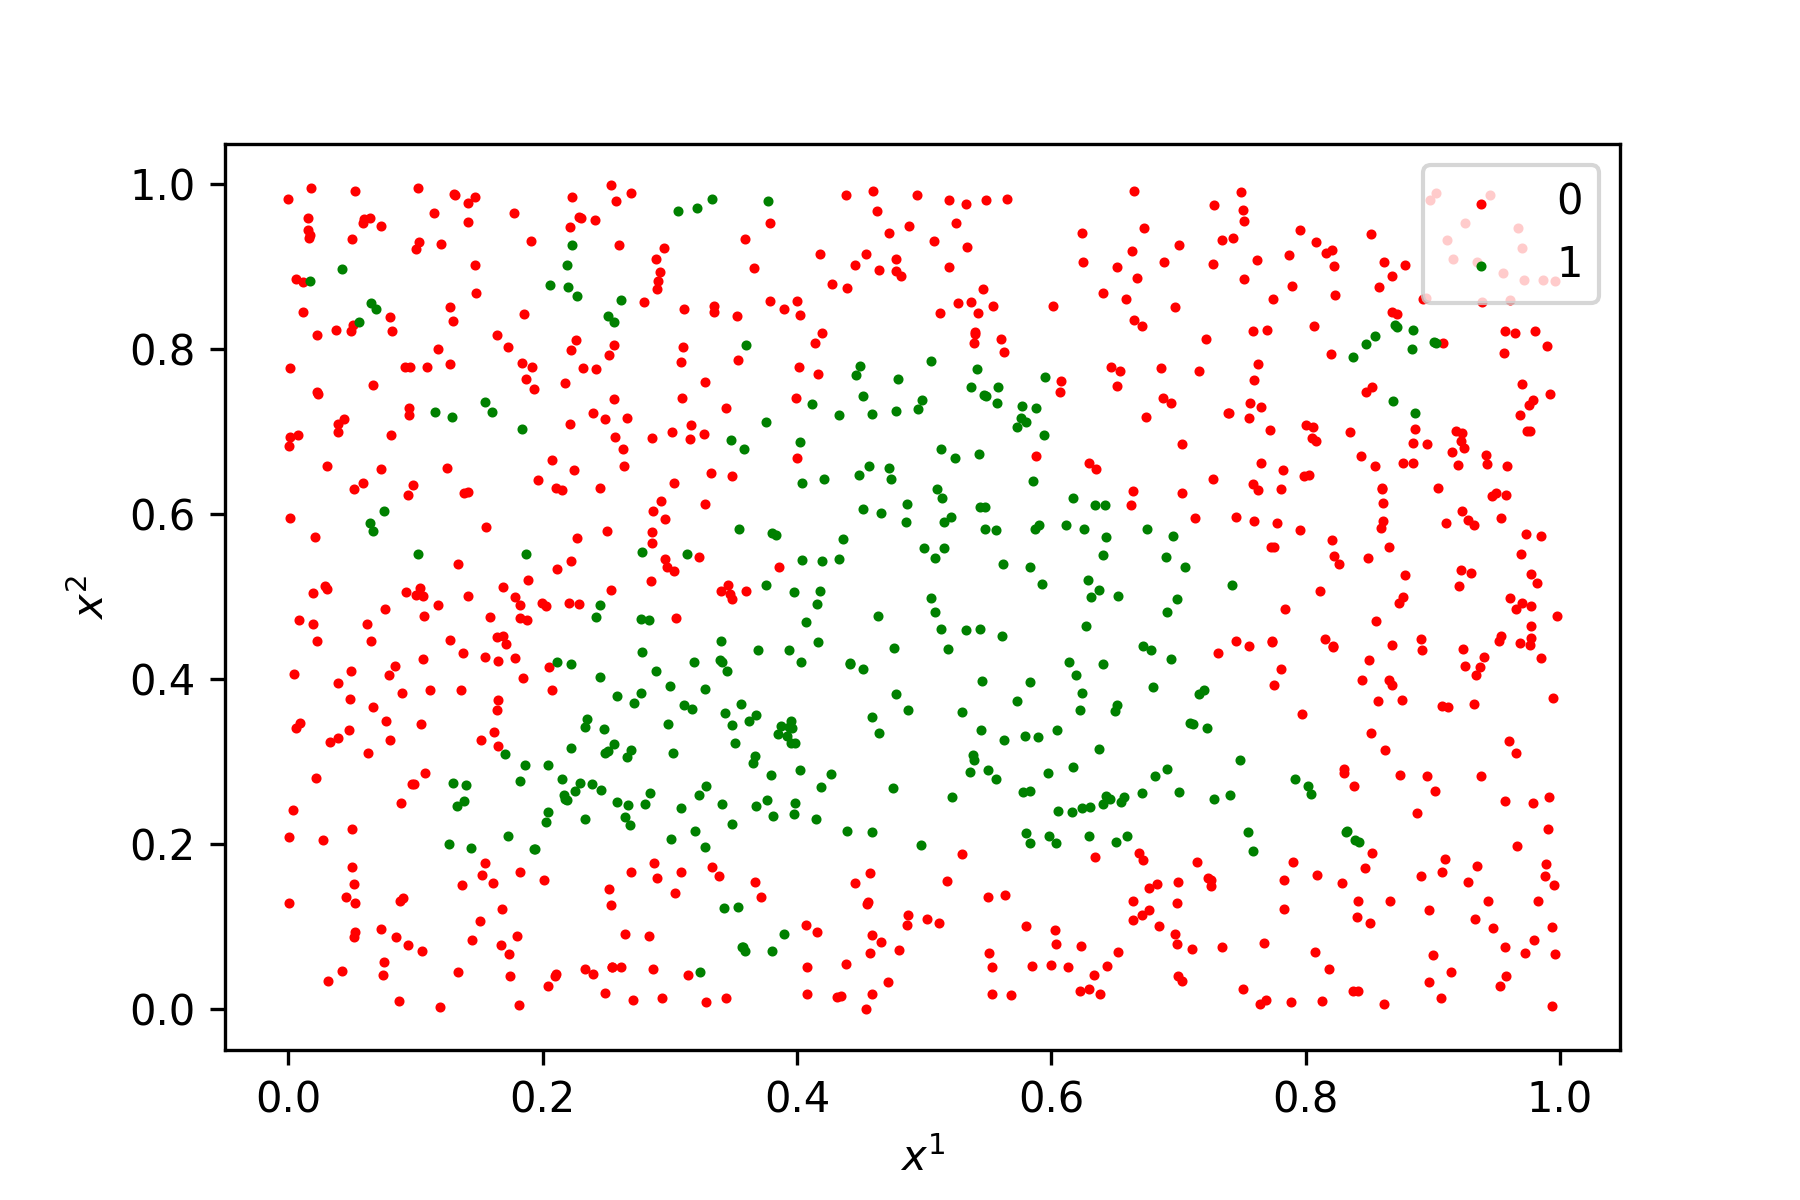
\includegraphics[width=\textwidth]{assets/ds_a.png}
  \caption{1,000 samples}
\end{subfigure}
\begin{subfigure}{.32\textwidth}
  \centering
  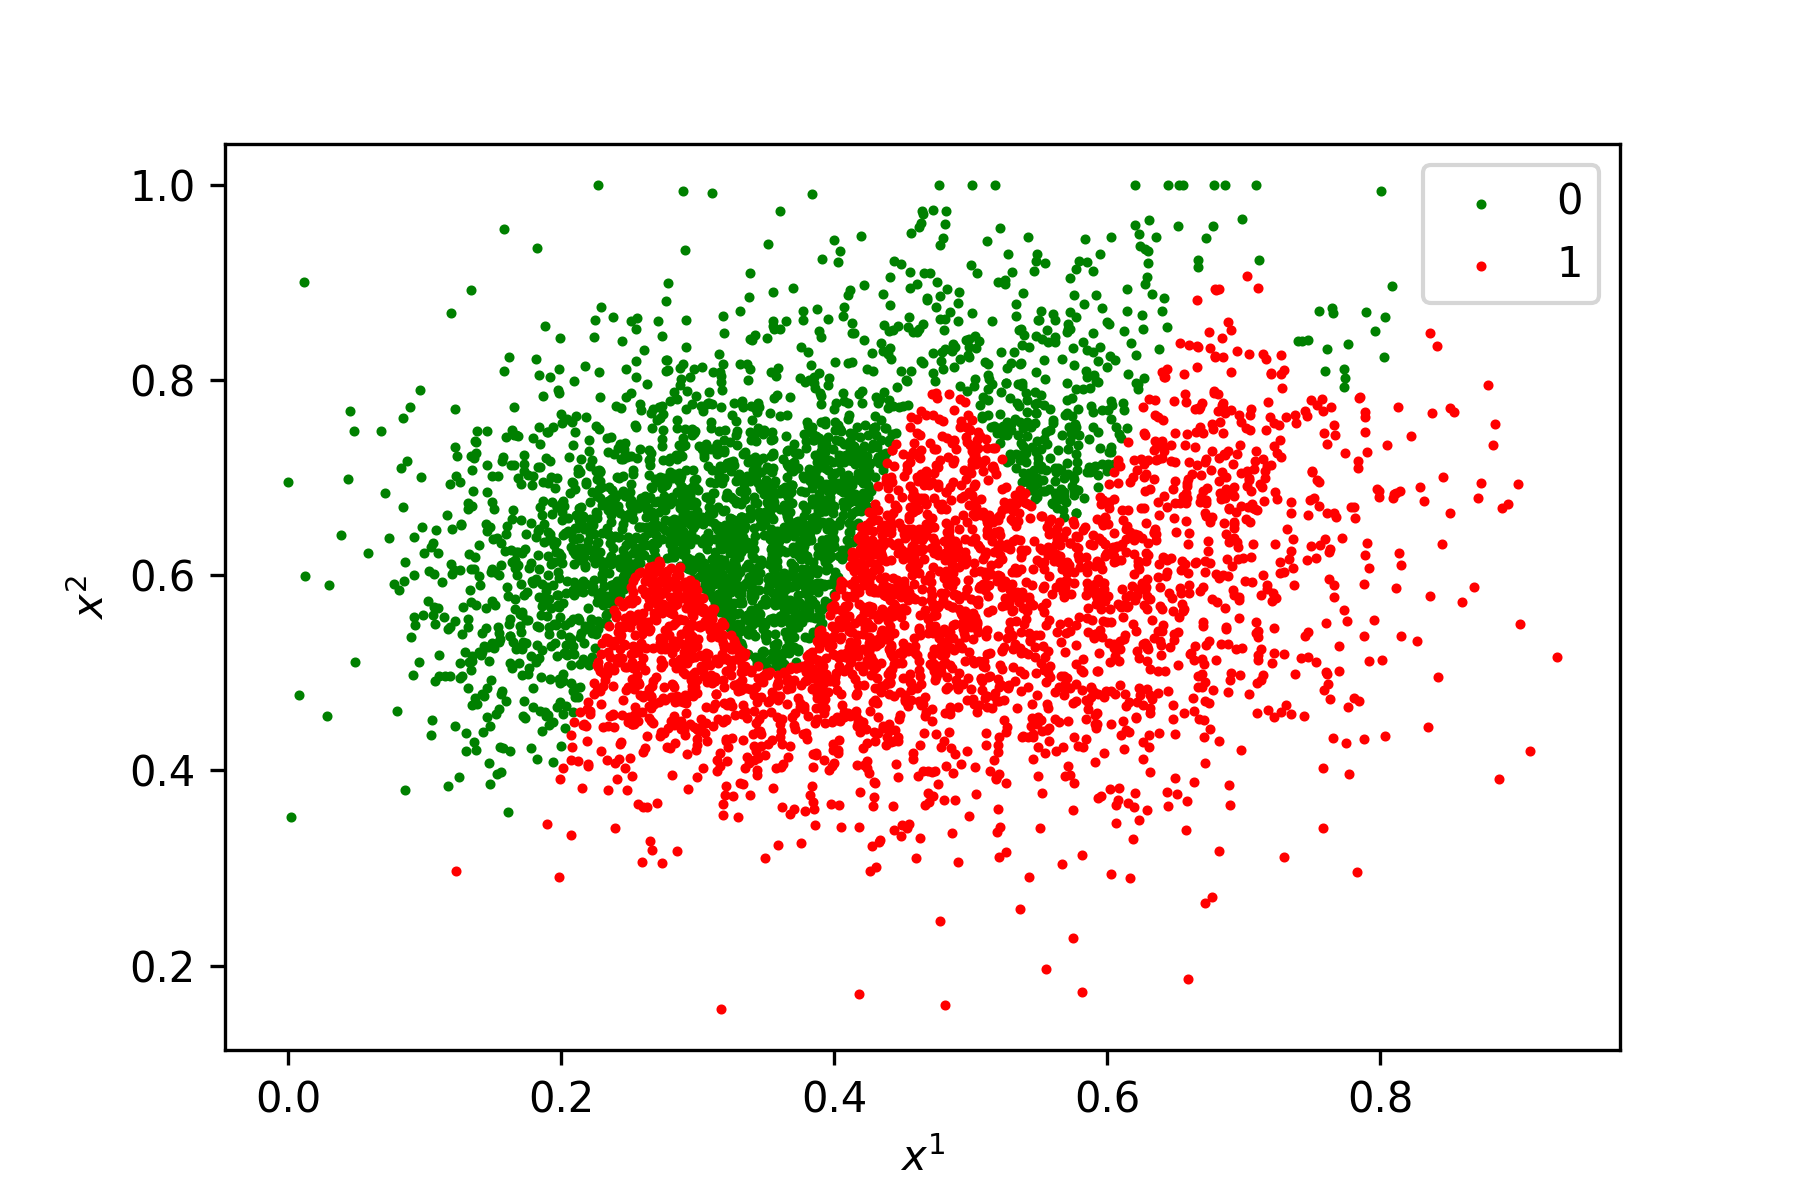
\includegraphics[width=\textwidth]{assets/ds_b.png}
  \caption{5,000 samples}
\end{subfigure}
\begin{subfigure}{.32\textwidth}
  \centering
  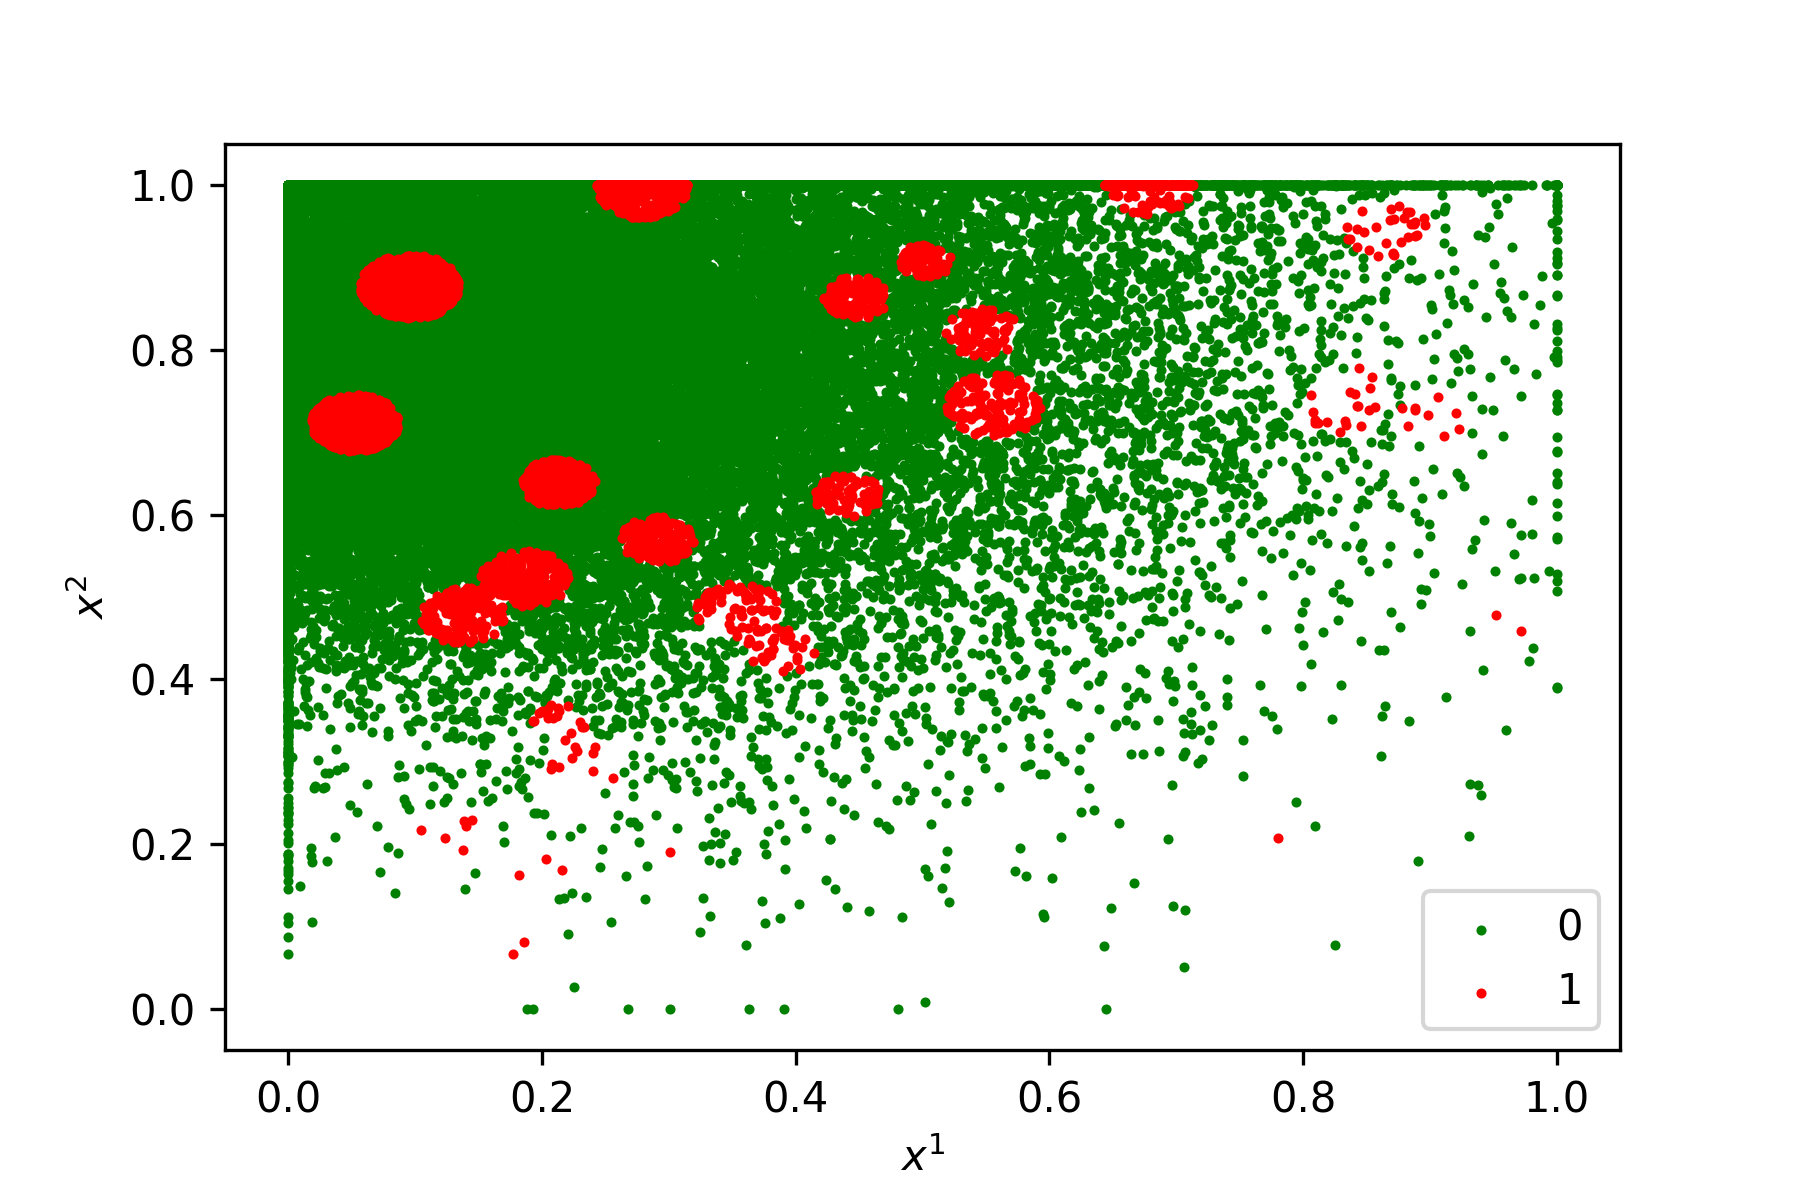
\includegraphics[width=\textwidth]{assets/ds_c.png}
  \caption{50,000 samples}
\end{subfigure}
\caption{The data sets of the challenge differ significantly in size, class balance and separability.}
\label{fig:datasets}
\end{figure}


\section{Possible Solutions and Related Work}

Before choosing an approach, we analysed the core aspect of safety guarantees and possible assumptions. In particular, we looked at two possibilities of formulating guarantees for our problem: (a) expressing uncertainty for a given sample and (b) robustness against local perturbations. 

The former addresses the problem that most machine learning approaches always produce an answer, even if they encounter inputs the like of which they have never seen before. In that case, they should be highly unsure about their prediction but mostly fail to express that. One way to counter this are Bayesian Neural Networks (BNNs) \cite{goan2020bnn}. In a probabilistic manner, they place a distribution over the network parameters. They can, hence, express their uncertainty in case they see challenging inputs. This could be very useful in a security-critical environment and would, for instance, allow an autonomous vehicle to alert its driver if it is unable to deal with a particular situation. However, it does not strictly correspond to the challenge description where security guarantees for \textit{unseen} inputs should be made. A BNN would require a concrete input $\mathbf{x}_i$ to express its certainty.

Therefore, we to decided pursue the goal of (b), meaning that we made our model robust against local perturbations. Simply put, this means that the model should reliably label unseen samples that lie near known training samples with the same class as the known sample. We put forward a more formal definition in Subsection \ref{ssec:verification}. 

It is trivial to give such guarantees for simple models: For logistic regression and k-nearest-neighbours, the decision boundary can be used to derive them. For naive Bayes classifiers, confidence intervals can be directly computed. Some of these classifiers would also perform relatively well on the given data sets, which is why we use them as baselines for our final model (see Subsection \ref{ssec:baselines}). However, they would not scale well to higher dimensions and more complex problems. 

More complicated models include support vector machines (SVM) and Gaussian Processes (GP) for classification. SVM can be powerful, especially with RBF kernels, but cannot provide the guarantees we require. GP would provide us with empirical confidence intervals but becomes inefficient in higher dimensions. Furthermore, both approaches are not leading in state-of-the-art predictive capabilities for challenging tasks, especially in the vision domain.

Another powerful class of machine learning models are decision trees and random forests. They display high predictive capabilities and can also be verified, but as \cite{tornblom2018formal} found, verification time does not scale very well to larger models.

Finally, we arrive at deep neural networks, which have received much attention in recent machine learning history. They scale well to very complex problems but used to be considered textbook examples for black-box models. However, recently, there has been a lot of work focused on explainability and defence against adversarial samples. It started with approaches that provided exact upper and lower bounds for neural network outputs given certain input perturbations. Reluplex \cite{katz2017reluplex} is an example that, however, only works for networks with ReLU activations. Further research introduced methods that work with arbitrary activations and use linear relaxations that compute tight approximations to significantly improve performance, allowing these techniques to be scaled to larger networks. Such work includes IBP \cite{gowal2019effectivenessIBP}, CROWN \cite{zhang2018efficient} and DeepPoly \cite{singh2019abstractDeepPoly}. We decided to use AutoLiRPA \cite{xu2020autoLiRPA}, a framework that applies these techniques to general neural networks and allows for automatic analysis on computational graphs.

\subsection{Baselines} \label{ssec:baselines}

To warrant the use of a complex deep neural network, we made sure that it exceeds the performance of simpler models. We established baselines with logistic regression \textit{(LR)}, Gaussian naive Bayes \textit{(NB)}, SVM with an RBF kernel \textit{(SVM)} and a gradient boosting classifier \textit{(GB)} as depicted in Table \ref{tab:baselines}. We observe that gradient boosting performs best for all data sets, followed by SVM. Data set A seems to be the most challenging one, probably due to the small sample size and irregular separability.

\begin{table}[]
\resizebox{\textwidth}{!}{%
\begin{tabular}{c|c|c|c|c|c|c|c|c|c|c|c|c|c|}
\cline{2-14}
\multicolumn{1}{l|}{}                                 & \textbf{Data set} & \multicolumn{4}{c|}{\textbf{A}}                          & \multicolumn{4}{c|}{\textbf{B}}                           & \multicolumn{4}{c|}{\textbf{C}}                          \\ \cline{2-14} 
\multicolumn{1}{l|}{}                                 & \textbf{Model}    & \textit{LR} & \textit{NB} & \textit{SVM} & \textit{GB}   & \textit{LR} & \textit{NB} & \textit{SVM} & \textit{GB}    & \textit{LR} & \textit{NB} & \textit{SVM} & \textit{GB}   \\ \hline
\multicolumn{1}{|c|}{\multirow{2}{*}{\textbf{Train}}} & Acc.              & 0.67        & 0.77        & 0.87         & \textbf{0.96} & 0.85        & 0.85        & 0.89         & \textbf{0.996} & 0.91        & 0.91        & 0.91         & \textbf{0.96} \\ \cline{2-14} 
\multicolumn{1}{|c|}{}                                & F1                & 0.81        & 0.73        & 0.87         & \textbf{0.96} & 0.85        & 0.85        & 0.89         & \textbf{0.996} & 0.95        & 0.95        & 0.95         & \textbf{0.96} \\ \hline
\multicolumn{1}{|c|}{\multirow{2}{*}{\textbf{Val}}}   & Acc.              & 0.67        & 0.75        & 0.84         & \textbf{0.92} & 0.88        & 0.88        & 0.90         & \textbf{0.984} & 0.91        & 0.91        & 0.91         & \textbf{0.96} \\ \cline{2-14} 
\multicolumn{1}{|c|}{}                                & F1                & 0.80        & 0.71        & 0.83         & \textbf{0.92} & 0.88        & 0.88        & 0.90         & \textbf{0.984} & 0.95        & 0.95        & 0.95         & \textbf{0.96} \\ \hline
\end{tabular}}
\caption{Results of baseline models}
\label{tab:baselines}
\end{table}

\section{Approach} \label{sec:approach}
%TODO
%• A description of the employed ML approach
%• All assumptions made, including an exhaustive proposal/justification for their validation


We model the safety criticality of our classifier's decisions using a cost matrix illustrated in Table~\ref{tab:cost_matrix}. Correctly classifying a sample obviously does not incur any cost, i.e. $c_{0,0} = c_{1,1} = 0$. In our particular example, assigning the label $0$ (green) to a data point with true label $1$ (red) is safety critical and therefore the associated cost $c_{1,0}$ should greatly exceed the cost $c_{0,1}$ of assigning the label $1$ (red) to true label $0$. Concrete values for $c_{0,1}$ and $c_{1,0}$ can be set by the users of our approach. The algorithm then minimises the total cost.

\begin{table}
  \begin{tabular}{|l|c|c|c|}\hline
    \backslashbox{True}{Predicted} & \makebox[3em]{0 (green)} & \makebox[3em]{1 (red)} \\ \hline
    0 (green) & $c_{0,0} = 0$ & $c_{0,1}$ \\ \hline
    1 (red) & $c_{1,0}$ & $c_{1,1} = 0$ \\\hline
  \end{tabular}
  \caption{Cost matrix for classifications}
  \label{tab:cost_matrix}
\end{table}

\subsection{Model} \label{ssec:model}

The model we use is a deep neural network implemented in PyTorch. It receives as input a 2D training sample, processes it through several hidden layers with ReLU activations and finally outputs a single scalar, activated through the sigmoid function $\sigma(a_i)$. If the output is smaller than 0.5, class 0 is assigned, class 1 otherwise. We use double weighted binary cross-entropy as our loss function:
\begin{equation}
	l_i = -w_{i}[py_{i} \log \sigma(a_i) + (1-y_i)\log(1-\sigma(a_i))]
\end{equation} 

where $l_i$ is the loss for sample $i$, $a_i$ is the output of the neural network before activated in sigmoid and $y_i$ is the correct label. To counter class imbalance, we set
\begin{equation}
w_i = \begin{cases}
\frac{\text{\# class 0 samples}}{\text{\# class 1 samples}} & y_i = 1\\
1 & y_i = 0.
\end{cases}
\end{equation}

This will cause the training samples of the underrepresented class to be weighted higher and thereby offset the imbalance. Additionally to that, we set the weight for positive examples $p = \frac{c_{1,0}}{c_{0,1}}$ to account for the costs of misclassification that differ per class. 

We train the model using Adam with learning rates around 0.0001 and a batch size of 32. % TODO still true?
To pick the best hyper-parameters, we use a validation set consisting of 20\% of all samples. The remaining 80\% of samples are used for training. Using the validation set, we can later also demonstrate our generalisation capabilities and ensure that we are not overfitting on the training set. 

\subsection{Verification} \label{ssec:verification}

Relying on the assumption that our training samples are correctly labelled, we want to guarantee for a certain number of samples, which we call \textit{verified}, that all inputs surrounding them are assigned the same class as the centre. Formally, we define a neighbourhood around training sample $\mathbf{x}_i$ as an $L_p$-ball with radius $\epsilon$. We then guarantee for all possible inputs that lie within this ball $B_\epsilon(\mathbf{x}_i) = \{\mathbf{y} \in \mathbb{R}: ||\mathbf{x}_i - \mathbf{y}||_p < \epsilon \}$ that they are assigned $l_i$. In our implementation, we support both the $L_2$ and the $L_\infty$-norm. Under the assumption that an unseen data point lies within the defined neighbourhood of a known training sample, we can give a probability that this new data point will be correctly classified based on the percentage of training samples that are verified. % TODO Let's talk about this sentence once more please.
We call this metric \textit{verified accuracy}. 

% TODO do we need some more justification for our use of the term "verified accuracy"? Prove it somehow or refer to another paper?
% TODO show what this looks like with a nice plot from data set A. Maybe two next to each other, one with L_2 and one with L_inf.

The challenging aspect of this verification is to show for all data points $\mathbf{y} \in B_\epsilon(\mathbf{x}_i)$ that they indeed are labelled with the same class as $\mathbf{x}_i$. As there exist infinitely many such inputs, it is impossible to let the model classify them all and check empirically. We, therefore, use the AutoLiRPA framework \cite{xu2020autoLiRPA} to compute bounds for the outputs of our network. To do so, we compute upper ($a_{\text{upper}}$) and lower ($a_{\text{lower}}$) bounds for every sample in our training data set, compute the respective sigmoid activations and check whether both the upper and the lower bound would result in the same prediction. If they do, we can guarantee that all inputs $\mathbf{y} \in B_\epsilon(\mathbf{x}_i)$ are classified as $l_i$. Otherwise, we cannot make that statement, and somewhere in the $\epsilon$-neighbourhood of $\mathbf{x_i}$ there exist inputs that our model would classify as $1-l_i$.

% TODO should we explain how autoLiRPA works a bit more?

\section{Experiments}
%TODO
% For each data set, an upper bound for the misclassification error, including its justification

% TODO write some generic stuff about our experiments. Exact model architecture?
% TODO W&B reference?

\subsection{Metrics}
In our experiments, we use a variety of different metrics, which allow us to compare the results given the imbalance of class labels in the data set as well as the safety-related cost associated with misclassification.

\begin{itemize}
	\item \textbf{Precision, Recall, F1}: For imbalanced models, precision, recall, F1 score are commonly used to compare the performance of classification models. They help capturing the trade-off between true-positive and false-positive predictions. 
	\item \textbf{Classification cost}: Our evaluation also captures the varying misclassification costs of the two classes as \textit{total classification cost}. It is defined as the sum of all misclassifications and their associated cost. Furthermore, we introduce the metric \textit{classification cost per sample} which allows us to compare the metric on datasets with a different number of samples. 
	\item \textbf{Verified Accuracy}: The verified accuracy which we introduced in Section~\ref{sec:approach} can quantify the probability of classifying an unseen data point correctly. This metric helps us to evaluate the dependability of our model.
\end{itemize}

In the end, we optimise our model for minimal classification cost. Depending on the $\epsilon$ chosen by the user, we achieve varying \textit{verified accuracies}.

\subsection{Architecture Search}
Due to the simplicity of the data sets we only use simple multilayer perceptron (MLP) architectures. We experiment with between one and three hidden layers and different number of neurons as well as regularization techniques such as weight decay and dropout regularization. To perform the architecture search we use the metric classification cost per sample, this metric helps us find a suitable model with respect to our security metrics. We utilize Weights \& Biases \cite{wandb} for tracking our experiments and for visualizing the results. 

\subsubsection*{Generalization}
A big problem for neural networks is overfitting. That is the network will end up fitting the training data very well, but will fail to generalize to new unseen data. To prevent this we use 20\% of the given data as validation data set. During training we monitor the validation loss and use early stopping to prevent the network from overfitting. 


\subsection{Results}

\subsubsection*{Data Set a}

\subsubsection*{Data Set b}

\begin{table}[]
  \resizebox{\textwidth}{!}{
  \begin{tabular}{cccllcllccc}
  \textbf{} & \multicolumn{1}{l}{} & \multicolumn{9}{l}{} \\ \cline{2-11} 
  \multicolumn{1}{c|}{} & \multicolumn{1}{c|}{\textbf{Cost}} & \multicolumn{3}{c|}{\textbf{1}} & \multicolumn{3}{c|}{\textbf{10}} & \multicolumn{3}{c|}{\textbf{50}} \\ \cline{2-11} 
  \multicolumn{1}{c|}{} & \multicolumn{1}{c|}{\textbf{$\epsilon$}} & \multicolumn{1}{c|}{\textbf{0.001}} & \multicolumn{1}{c|}{\textbf{0.01}} & \multicolumn{1}{c|}{\textbf{0.025}} & \multicolumn{1}{c|}{\textbf{0.001}} & \multicolumn{1}{c|}{\textbf{0.01}} & \multicolumn{1}{c|}{\textbf{0.025}} & \multicolumn{1}{c|}{\textbf{0.001}} & \multicolumn{1}{c|}{\textbf{0.01}} & \multicolumn{1}{c|}{\textbf{0.025}} \\ \hline
  \multicolumn{1}{|c|}{\textbf{Full}} & \multicolumn{1}{c|}{\textbf{Verified Acc.}} & \multicolumn{1}{l|}{0.9864} & \multicolumn{1}{l|}{0.8804} & \multicolumn{1}{l|}{0.6836} & \multicolumn{1}{l|}{0.9854} & \multicolumn{1}{l|}{0.8880} & \multicolumn{1}{l|}{0.7052} & \multicolumn{1}{c|}{0.9760} & \multicolumn{1}{c|}{0.8802} & \multicolumn{1}{c|}{0.6514} \\ \hline
  \multicolumn{1}{|c|}{\multirow{3}{*}{\textbf{Train}}} & \multicolumn{1}{c|}{\textbf{Acc.}} & \multicolumn{3}{c|}{0.9915} & \multicolumn{3}{c|}{0.9918} & \multicolumn{3}{c|}{0.9810} \\ \cline{2-11} 
  \multicolumn{1}{|c|}{} & \multicolumn{1}{c|}{\textbf{F1}} & \multicolumn{3}{c|}{0.9859} & \multicolumn{3}{c|}{0.9813} & \multicolumn{3}{c|}{0.9521} \\ \cline{2-11} 
  \multicolumn{1}{|c|}{} & \multicolumn{1}{l|}{\textbf{Cost/Sample}} & \multicolumn{3}{c|}{0.0085} & \multicolumn{3}{c|}{0.0105} & \multicolumn{3}{c|}{0.0190} \\ \hline
  \multicolumn{1}{|l|}{\multirow{3}{*}{\textbf{Val}}} & \multicolumn{1}{c|}{\textbf{Acc.}} & \multicolumn{3}{c|}{0.9880} & \multicolumn{3}{c|}{0.9890} & \multicolumn{3}{c|}{0.9850} \\ \cline{2-11} 
  \multicolumn{1}{|l|}{} & \multicolumn{1}{c|}{\textbf{F1}} & \multicolumn{3}{c|}{0.9888} & \multicolumn{3}{c|}{0.9892} & \multicolumn{3}{c|}{0.9869} \\ \cline{2-11} 
  \multicolumn{1}{|l|}{} & \multicolumn{1}{l|}{\textbf{Cost/Sample}} & \multicolumn{3}{c|}{0.0012} & \multicolumn{3}{c|}{0.029} & \multicolumn{3}{c|}{0.015} \\ \hline
  \end{tabular}}
  \end{table}

\subsubsection*{Data Set c}


\section{Discussion}
%TODO
% An outline how the approach could be scaled to higher dimensions

%- quick summary of our method (this is the conclusion!)
%
%- Advantages
%  - scaling to higher dimensions (esp. images, transformer)
%    - complex architectures
%  - high predictive capabilities
%  - verifications for perturbations
%  - very performant compared to exact perturbation methods (e.g. Reluplex)
%- Limitations
%  - assumptions have to be made
%  - compared to simple models, more resource-intense to train (but that's the price you have to pay for good results 😎)


\pagebreak  

%%
%% The next two lines define the bibliography style to be used, and
%% the bibliography file.
\bibliographystyle{ACM-Reference-Format}

\bibliography{references}
% References to results that are used


\end{document}
\endinput

